\documentclass[11pt]{article}

\usepackage[utf8]{inputenc}
\usepackage[T1]{fontenc}
\usepackage[margin=1in]{geometry}
\usepackage{amsmath,amssymb}
\usepackage{booktabs}
\usepackage{graphicx}
\usepackage{xcolor}
\usepackage{hyperref}
\usepackage{multirow}
\usepackage{array}
\usepackage{caption}
\usepackage{authblk}
\usepackage{algorithm}
\usepackage{algpseudocode}
\usepackage{enumitem}

\hypersetup{
  colorlinks=true,
  linkcolor=blue!55!black,
  citecolor=blue!55!black,
  urlcolor=blue!55!black
}

\newcommand{\ebar}{\bar{e}}
\newcommand{\compose}{\textsc{compose}}
\newcommand{\decompose}{\textsc{decompose}}
\newcommand{\R}{\mathbf{R}}

\title{\textbf{Compositional Token Algebra: Reversible, Session-Scoped\\
Deduplication of Repeated Spans for Compute-Aware Transformers}}

\author{}
\date{}

\begin{document}

\maketitle
\vspace{-2.5em}
\begin{center}
\textit{Preprint. Work in progress.}
\end{center}
\vspace{1em}

\begin{abstract}
Modern language models treat the token as a unit of \emph{text} rather than a unit of
\emph{computation}: every occurrence of a repeated identifier, boilerplate line, or
duplicated system prompt pays the full quadratic attention cost anew, regardless of how
predictable it is. We introduce \textbf{Compositional Token Algebra (CTA)}, a
parameter-free, \emph{reversible} layer that detects repeated spans \emph{within a single
context} (session-scoped), collapses each span into a single pooled vector via a
deterministic operator \compose, and---crucially---can reconstruct the original token
embeddings exactly via an inverse operator \decompose. Because collapse is lossless by
construction, a small learnable \emph{expand-gate} can decide, per span, whether the
collapsed representation is sufficient (cheap, opaque) or must be expanded back to full
resolution (expensive, transparent), trading attention FLOPs against fidelity on a
per-span basis. On a frozen GPT-2, we show (i) reconstruction error at machine epsilon
($\sim\!5\times10^{-7}$); (ii) on code, a naive always-collapsed pass reaches $12.3\%$ of
baseline attention FLOPs, and a gated variant reaches $\sim\!50\%$ FLOPs while
\emph{improving} perplexity by $11.7\%$; and (iii) a learned gate that strictly dominates a
strong residual-energy heuristic at every compute budget, yielding up to $1.09$ nats
(code) and $1.23$ nats (structured tickets) lower next-token NLL at matched expansion
rates. Beyond FLOPs, we report measured end-to-end wall-clock: on CPU the realized
speedup is ${\sim}1.5\times$ and \emph{grows with sequence length}
($1.29\times\!\to\!1.71\times$ over $256\!\to\!1024$ tokens), since only the quadratic
attention term shrinks while MLP/head costs stay length-linear; as a lossless side
effect, collapse extends the effective context window by ${\sim}1.9\times$ on
repetition-heavy input. The mechanism ports unchanged to a modern architecture: on
Qwen2.5-0.5B (RoPE + GQA, 32k window) reversibility holds at ${\sim}4\times10^{-9}$ and the
speedup likewise grows with length (up to $1.58\times$ at 2048 tokens). We position CTA against ASG, R3Mem, H-Net, and Token Merging, and argue it occupies
a previously empty niche: the only \emph{reversible, session-scoped, parameter-free}
deduplication mechanism motivated by compute amortization rather than compression. We close
with an honest characterization of its applicability boundary: CTA is a clear win on
\emph{deep} redundancy (code, boilerplate) and requires aggressive gated expansion on
\emph{shallow} redundancy (structured logs) where repeated field templates immediately
precede distinguishing content.
\end{abstract}

\section{Introduction}
\label{sec:intro}

Tokenization and attention are usually developed in isolation: the tokenizer is a fixed
preprocessing stage, and attention is the model. As a consequence, the token is
implicitly defined as a \emph{unit of text}, and the computational cost of a sequence
scales with its textual length regardless of the information content of that text. This
is wasteful whenever the input contains \emph{repeated spans}: a codebase repeats
\texttt{import} statements, function signatures, and idiomatic bodies; structured logs
repeat field templates; multi-turn conversations repeat a system prompt before every
turn. Each repetition re-enters the $O(n^2)$ attention computation as if it were novel.

A growing line of work reframes the token as a \emph{unit of computation}. Byte Latent
Transformer (BLT)~\cite{blt} allocates compute by entropy: predictable byte stretches are
grouped into long patches, unpredictable ones into short patches, redistributing FLOPs to
where the data is hard. H-Net~\cite{hnet} learns hierarchical chunk boundaries end-to-end.
These methods adapt \emph{granularity} to \emph{local difficulty}. They do not, however,
exploit \emph{global repetition}: two identical spans far apart in the context are each
processed at full cost.

Orthogonally, prompt/prefix caching amortizes a \emph{shared prefix} across requests, but
cannot compress repeats that occur in the \emph{interior} of a single context, and does
not give repeated content any reusable identity. Token merging (ToMe)~\cite{tome} and
KV-cache compression reduce sequence length on the fly, but do so \emph{lossily}: merged
tokens cannot be recovered.

We propose to close this gap with \textbf{Compositional Token Algebra (CTA)}. The central
design commitment is \emph{reversibility}: rather than merging a repeated span into a
single vector destructively, we define a deterministic, parameter-free pair of operators
$(\compose, \decompose)$ such that $\decompose(\compose(x)) = x$ exactly. The collapsed
representation stores a centroid; a side ``residual store'' holds the deviations. Because
no information is lost, the model is free to operate on the compact collapsed sequence by
default (Level~0, \emph{opaque}), and to \emph{expand} a span back to full resolution only
when a query genuinely needs its internals (Level~1, \emph{transparent}). The decision is
made by a small learnable gate $\gamma(q, \ebar)$ trained with a compute-aware objective
that explicitly penalizes expansions.

\paragraph{Contributions.}
\begin{enumerate}[leftmargin=1.4em,itemsep=1pt]
  \item \textbf{A reversible span algebra.} Parameter-free $(\compose, \decompose)$ with
  exact reconstruction ($\sim\!5\times10^{-7}$ on real GPT-2 embeddings,
  Section~\ref{sec:reversibility}).
  \item \textbf{A gated compute/quality frontier.} We show the opaque failure mode is
  content-driven, not positional, and that selective expansion recovers and even exceeds
  baseline quality on code at $\sim\!50\%$ attention FLOPs (Section~\ref{sec:frontier}).
  \item \textbf{A learnable, compute-aware gate.} A small MLP with a Gumbel-Sigmoid
  relaxation and a sparsity regularizer strictly dominates a residual-energy heuristic at
  every budget, by up to $1.23$ nats (Section~\ref{sec:gate}).
  \item \textbf{Positioning.} We argue CTA is the unique reversible, session-scoped,
  parameter-free deduplication method (Section~\ref{sec:related}), and we delineate its
  applicability boundary (Section~\ref{sec:conclusion}).
\end{enumerate}

\section{Related Work}
\label{sec:related}

We position CTA along four axes: does the method \emph{compose} tokens; is the composition
\emph{reversible}; is it \emph{session-scoped / on-the-fly}; and what \emph{motivates} it.
Table~\ref{tab:related} summarizes the comparison.

\paragraph{Aggregate Semantic Grouping (ASG)~\cite{asg}.} ASG compresses the embedding
table by mapping tokens to ``ConceptIDs'' via Product Quantization. The mapping is
\emph{global}, \emph{precomputed}, and \emph{non-reversible}: it is designed to reduce
parameters, not to amortize per-context computation, and it cannot recover the original
token from a ConceptID. CTA shares the word ``compositional'' but differs on every axis:
it is session-scoped, reversible, and motivated by compute amortization.

\paragraph{R3Mem~\cite{r3mem}.} R3Mem is the closest prior work on \emph{reversibility}: it
compresses and reconstructs long-context memory via a reversible ``zip/unzip''
architecture. However, it is \emph{parametric} (trained adapters) and targets long-context
retrieval and memory, not the deduplication of lexical/semantic repeats within a context.
CTA's reversibility is instead a property of a \emph{parameter-free} algebraic
construction (centroid $+$ residual).

\paragraph{H-Net~\cite{hnet} and Dynamic Token Pooling~\cite{dtp}.} Both learn where to
place chunk/pool boundaries and adapt granularity to difficulty. Neither is reversible
(pooling is lossy), and neither deduplicates \emph{repeated} spans: two identical spans are
pooled independently, each at full upstream cost. CTA is complementary---it can sit atop a
byte/patch tokenizer such as BLT or H-Net, treating patches as its atoms.

\paragraph{Token Merging (ToMe)~\cite{tome} and KV compression.} ToMe merges similar tokens
on the fly to raise throughput, but merges are lossy and permanent. CTA's collapse is
information-preserving: any collapsed span can be losslessly restored, enabling the
per-query granularity choice that lossy merging forecloses.

\begin{table}[t]
\centering
\caption{Positioning of CTA against related methods. CTA is the only method that is
simultaneously reversible, session-scoped, parameter-free, and motivated by compute
amortization on repeated spans.}
\label{tab:related}
\small
\begin{tabular}{lccccl}
\toprule
\textbf{Method} & \textbf{Composes} & \textbf{Reversible} & \textbf{Session-scoped} & \textbf{Param-free} & \textbf{Motivation} \\
\midrule
ASG~\cite{asg}            & \checkmark & $\times$ & $\times$ & $\times$ & Parameter compression \\
R3Mem~\cite{r3mem}        & \checkmark & \checkmark & $\times$ & $\times$ & Long-context memory \\
Dyn. Pooling~\cite{dtp}   & \checkmark & $\times$ & partial  & $\times$ & Efficiency \\
H-Net~\cite{hnet}         & \checkmark & $\times$ & learned  & $\times$ & Tokenizer-free \\
ToMe~\cite{tome}          & \checkmark & $\times$ & \checkmark & \checkmark & Throughput \\
\textbf{CTA (ours)}       & \checkmark & \checkmark & \checkmark & \checkmark & \textbf{Compute amortization} \\
\bottomrule
\end{tabular}
\end{table}

\section{Compositional Token Algebra}
\label{sec:method}

\subsection{Operators}

Let the context be a sequence of token embeddings $X = (x_1,\dots,x_n)$, $x_i \in
\mathbb{R}^d$. A span $s = (x_a,\dots,x_b)$ of length $k = b-a+1$ is a contiguous segment.

\paragraph{\compose\ (parameter-free).}
\begin{equation}
\compose(s) = (\ebar_s, \R_s), \qquad
\ebar_s = \sum_{i=a}^{b} \pi_i\, x_i,\quad
\pi_i = \frac{\exp(g(x_i))}{\sum_{j=a}^{b}\exp(g(x_j))},
\end{equation}
where $g(\cdot)$ is a \emph{fixed}, non-trainable scoring function
(Section~\ref{sec:scoring}), $\pi$ is a positional pooling distribution, $\ebar_s$ is the
collapsed embedding, and
\begin{equation}
\R_s = \big(x_i - \ebar_s\big)_{i=a}^{b}
\end{equation}
is the residual store, held \emph{outside} the attention context so it does not enter the
$O(n^2)$ cost.

\paragraph{\decompose\ (exact inverse).}
\begin{equation}
\decompose(\ebar_s, \R_s) = \big(\ebar_s + \R_{s,i}\big)_{i=a}^{b} = (x_a,\dots,x_b).
\end{equation}
Reversibility is exact by construction: the centroid plus its deviations reconstruct the
input, independent of the choice of $g$. Unlike Reformer-style reversible layers or R3Mem,
no learned inverse is required.

\subsection{Why ``algebra''}
The operators form a structure rather than a one-shot pooling step: (i) composition is
\emph{associative}, enabling hierarchical composition of adjacent spans while remaining
reversible at each level; (ii) \decompose\ admits a \emph{partial} form restoring only a
requested sub-range $[c,d]\subseteq[a,b]$, giving per-query granularity; and (iii) on
near-duplicate spans $s'\approx s$ we have $\ebar_{s'}\approx\ebar_s$, so residuals can
reference a shared centroid, which is precisely the compute-amortization mechanism.

\subsection{Fixed scoring functions}
\label{sec:scoring}
We consider four parameter-free choices for $g$, used as ablations:
(1) \emph{uniform} ($g\equiv 0$, mean pooling);
(2) \emph{norm-weighted} ($g(x_i)=\lVert x_i\rVert$);
(3) \emph{positional-decay} ($g(x_i)=-\lambda(b-i)$, emphasizing the right boundary);
(4) \emph{self-consistency} ($g(x_i)=\langle x_i,\bar{x}\rangle$).

\subsection{The attention-transparency problem and the expand-gate}
\label{sec:transparency}
If a span is collapsed to a single token, how does the rest of the context attend to its
\emph{internal} positions? CTA resolves this with a per-query choice of granularity:
\begin{description}[leftmargin=1.4em,itemsep=1pt]
  \item[Level 0 --- Opaque (default, cheap).] A query attends to $\ebar_s$ as a single
  token: $1$ position instead of $k$. This is where attention FLOPs are actually saved.
  \item[Level 1 --- Gated expand (on demand).] A scalar gate
  $\gamma(q,\ebar_s)\in[0,1]$ decides whether to \decompose\ the span for this query; if
  $\gamma>\tau$ the query attends to the $k$ internal positions, otherwise the span stays
  opaque.
  \item[Level 2 --- Partial expand.] The gate designates a sub-range of interest, yielding
  partial \decompose. (Not evaluated here.)
\end{description}
The expected attention cost is
$\mathbb{E}[\text{cost}] = n_{\text{collapsed}} + \sum_s \Pr[\gamma_s>\tau]\cdot k_s$,
so savings are realized precisely when repeats are rarely expanded.

\subsection{Learnable gate}
\label{sec:gate-arch}
We instantiate $\gamma$ as a small MLP over parameter-free features:
$\big[\,q \,\Vert\, \ebar_s \,\Vert\, \lVert\R_s\rVert_F \,\Vert\, k\,\big]
\to \text{Linear}(128)\to\text{GELU}\to\text{Linear}(1)$,
where $q$ is the ``consumer query'' (the embedding of the token immediately following the
span, i.e.\ the position that must predict the next token using this span as context). The
backbone transformer is \emph{frozen}; only the gate ($\sim\!2\times10^5$ parameters) is
trained. Discreteness of the expand decision is handled by a Gumbel-Sigmoid (binary
concrete) relaxation with straight-through estimation at evaluation.

\paragraph{Compute-aware objective.}
For span $i$ with expand probability $p_i=\sigma_{\text{GS}}(\gamma_i)$,
\begin{equation}
\label{eq:loss}
\mathcal{L} = \underbrace{\frac{1}{N}\sum_{i}\Big[p_i\,\mathrm{NLL}^{\text{exp}}_i +
(1-p_i)\,\mathrm{NLL}^{\text{pool}}_i\Big]}_{\text{task / cross-entropy proxy}}
\;+\; \lambda \underbrace{\frac{1}{N}\sum_i p_i}_{\text{sparsity (FLOPs) regularizer}} .
\end{equation}
Here $\mathrm{NLL}^{\text{pool}}_i$ and $\mathrm{NLL}^{\text{exp}}_i$ are the next-token
negative log-likelihoods of the post-span target when span $i$ is pooled vs.\ expanded
(all other spans pooled), precomputed once with the frozen backbone. Sweeping $\lambda$
traces the compute/quality frontier.

\subsection{Span detection and collapse policy}
Repeated spans are found online with a rolling hash over token-id windows (an $O(n)$
amortized suffix-automaton is an alternative). A span is a collapse candidate when
$\mathrm{freq}(s)\ge f_{\min}$ and $k\ge k_{\min}$; a greedy non-overlapping selection
favors long, frequent spans. In all experiments we use $k_{\min}=3$, $k_{\max}=16$,
$f_{\min}=2$.

\section{Experimental Setup}
\label{sec:setup}

All experiments use a \emph{frozen} GPT-2 small (124M parameters, $12$ layers, $d=768$),
CPU, inference-only for the backbone. Attention FLOPs are reported as a proxy
$\sum_{\text{layers}} 2 L^2 d$, so a sequence-length reduction $n\to m$ yields a
$(m/n)^2$ attention-cost ratio. To keep collapsed and baseline sequences comparable, we
add positional embeddings over the (possibly collapsed) sequence positions in both cases;
a control that instead preserved original ``anchor'' positions performed \emph{worse}
(Section~\ref{sec:frontier}), confirming that compressed positions are the correct choice.

\paragraph{Data.} We use three families with differing redundancy structure:
\emph{code} (real Python from \texttt{requests}, \texttt{flask}, \texttt{click},
CPython), \emph{structured logs / tickets} (JSON log lines and Jira-style tickets with
repeated field templates), and \emph{multi-turn chat} with a repeated system prompt. A
low-repetition prose control yields no collapse candidates, confirming CTA is inert
without repetition.

\paragraph{Evaluation protocol.} Baseline and CTA predict the \emph{same} original target
tokens: the first token of each segment following at least one collapsed span. At these
positions the baseline attends to the full repeated span while CTA attends to the pooled
token, directly testing whether context compression harms next-token prediction.

\section{Reversibility}
\label{sec:reversibility}

Over $800$ random spans across all four scoring functions and on real GPT-2 embeddings,
the maximum reconstruction error $\max_i\lVert\decompose(\compose(x))_i - x_i\rVert_\infty$
was $4.77\times10^{-7}$, i.e.\ at float32 machine epsilon (Table~\ref{tab:reversibility}).
Reversibility is thus a verified property, not an approximation.

\begin{table}[h]
\centering
\caption{Maximum reconstruction error of $\decompose\circ\compose$ by scoring function
(float32).}
\label{tab:reversibility}
\small
\begin{tabular}{lcccc}
\toprule
Scoring $g$ & uniform & norm & pos-decay & self-consist. \\
\midrule
Max $\ell_\infty$ error & $2.4\times10^{-7}$ & $4.8\times10^{-7}$ & $4.8\times10^{-7}$ & $4.8\times10^{-7}$ \\
\bottomrule
\end{tabular}
\end{table}

\section{The Opaque Failure Mode and the Gated Frontier}
\label{sec:frontier}

\paragraph{Naive opaque collapse.} With every repeated span collapsed and never expanded,
attention FLOPs drop dramatically---to $12.3\%$ (code), $3.0\%$ (logs), and $4.2\%$
(chat) of baseline---but quality diverges on shallow-redundancy data
(Table~\ref{tab:opaque}). A diagnostic that preserved original anchor positions made
matters \emph{worse} (e.g.\ code perplexity $38.9\to98.6$), isolating the cause as
\emph{content opacity}: collapsing destroys span-internal information that the immediately
following token depends on. This motivates the gate.

\begin{table}[h]
\centering
\caption{Naive always-opaque collapse: large FLOPs savings but content-dependent quality.
$\Delta$PPL is relative to baseline at the same eval positions.}
\label{tab:opaque}
\small
\begin{tabular}{lccccc}
\toprule
Data & $n\!\to\!m$ & Attn.\ FLOPs & Base PPL & CTA PPL & $\Delta$PPL \\
\midrule
code & $394\!\to\!138$ & $12.3\%$ & $33.63$ & $38.95$ & $+15.8\%$ \\
logs & $232\!\to\!40$  & $3.0\%$  & $3.57$  & $246.95$ & $+6810\%$ \\
chat & $131\!\to\!27$  & $4.2\%$  & $3.65$  & $592.83$ & $+16165\%$ \\
\bottomrule
\end{tabular}
\end{table}

\paragraph{Gated frontier (heuristic gate).} Expanding the top fraction of spans by
residual energy $\lVert\R_s\rVert_F$ traces a compute/quality frontier
(Table~\ref{tab:frontier}). On code, a $25\%$ expansion budget reaches $49.8\%$ of
baseline attention FLOPs while \emph{improving} perplexity by $11.7\%$: code repeats are
genuinely redundant, so pooling most of them loses nothing predictive. Logs and chat
require $\sim\!75\%$ expansion before quality recovers, because their ``repeats'' (e.g.\
\texttt{"user\_id":}) immediately precede distinguishing content.

\begin{table}[h]
\centering
\caption{Residual-energy gated frontier. Code admits large savings at improved quality;
logs/chat are expansion-hungry.}
\label{tab:frontier}
\small
\begin{tabular}{llcccc}
\toprule
Data & Expand budget & Spans expanded & Attn.\ FLOPs & CTA PPL & $\Delta$PPL vs base \\
\midrule
\multirow{3}{*}{code}
 & $0\%$   & $0/66$  & $12.3\%$ & $38.95$ & $+15.8\%$ \\
 & $25\%$  & $16/66$ & $49.8\%$ & $29.69$ & $\mathbf{-11.7\%}$ \\
 & $50\%$  & $33/66$ & $69.3\%$ & $24.82$ & $\mathbf{-12.3\%}$ \\
\midrule
\multirow{3}{*}{logs}
 & $0\%$   & $0/24$  & $3.0\%$  & $246.95$ & $+6810\%$ \\
 & $50\%$  & $12/24$ & $71.4\%$ & $49.64$  & $+1289\%$ \\
 & $75\%$  & $18/24$ & $89.9\%$ & $4.89$   & $+52.3\%$ \\
\midrule
\multirow{3}{*}{chat}
 & $25\%$  & $3/12$  & $30.2\%$ & $72.09$  & $+1792\%$ \\
 & $50\%$  & $6/12$  & $61.8\%$ & $10.34$  & $+209.7\%$ \\
 & $75\%$  & $9/12$  & $86.7\%$ & $3.37$   & $+87.6\%$ \\
\bottomrule
\end{tabular}
\end{table}

\begin{figure}[t]
\centering
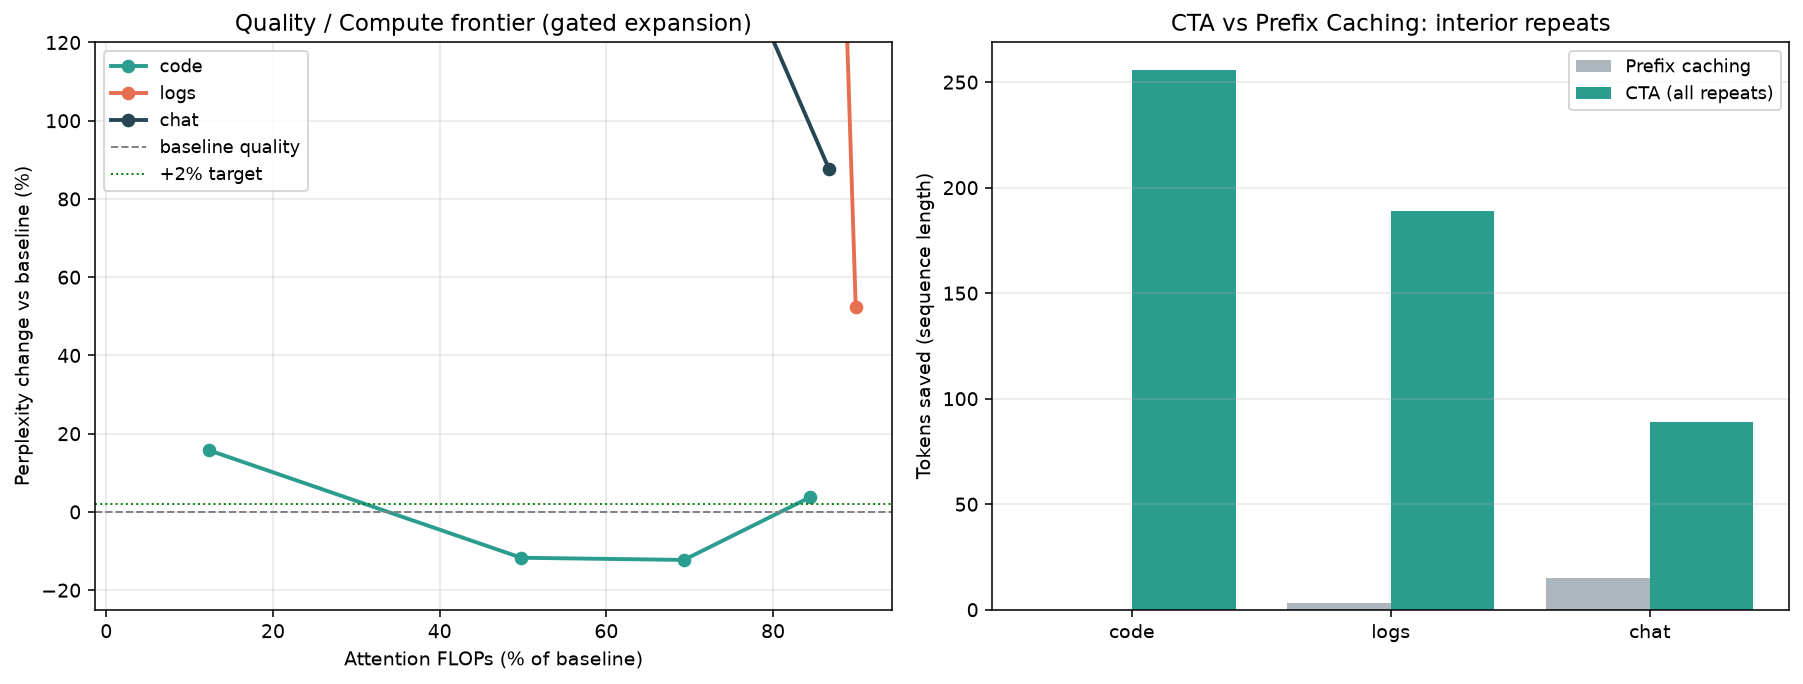
\includegraphics[width=0.92\textwidth]{cta_results.png}
\caption{Left: quality/compute frontier under the residual-energy gate; code (teal) dips
below baseline quality at $\sim\!50\%$ FLOPs, while logs/chat remain expansion-hungry.
Right: CTA vs.\ prefix caching. Prefix caching captures only prefix repeats ($0/3/15$
tokens); CTA additionally captures interior repeats ($256/192/104$ tokens) that prefix
caching structurally cannot.}
\label{fig:frontier}
\end{figure}

\paragraph{CTA vs.\ prefix caching.} Prefix caching amortizes only a shared prefix. On our
interior-repeat data it saves $0$ (code), $3$ (logs), and $15$ (chat) tokens, whereas CTA
saves $256$, $192$, and $104$ tokens respectively---almost entirely interior repeats that
prefix caching cannot reach (Figure~\ref{fig:frontier}, right). This is CTA's defensible
niche.

\section{Learned Gate}
\label{sec:gate}

We train the MLP gate of Section~\ref{sec:gate-arch} on cached per-span outcomes with the
objective in Eq.~\eqref{eq:loss}, sweeping the sparsity weight $\lambda$. We compare
against the residual-energy heuristic \emph{at matched expansion budgets}.

\paragraph{Redundancy diagnostic.} The average harm of pooling
($\mathrm{NLL}^{\text{pool}}-\mathrm{NLL}^{\text{exp}}$) is $0.133$ nats on code versus
$3.063$ nats on tickets---a $23\times$ gap that quantifies the deep-vs-shallow redundancy
distinction and predicts that a good gate should expand few code spans but many ticket
spans.

\paragraph{The learned gate strictly dominates the heuristic.} At every budget on both
datasets the learned gate achieves lower next-token NLL (Table~\ref{tab:gate},
Figure~\ref{fig:gate}). On code it reaches NLL $5.06$ at $37.5\%$ expansion---\emph{below}
the all-expanded NLL of $6.03$---by learning which spans matter. On tickets it correctly
refuses sparsity at small $\lambda$ (pooling is costly there) and, when forced to $42.5\%$
expansion, still beats the heuristic by $1.23$ nats.

\begin{table}[h]
\centering
\caption{Learned gate vs.\ residual-energy heuristic at matched expansion budgets.
Backbone frozen; only the gate is trained. Gain $=$ heuristic NLL $-$ learned NLL (nats,
higher is better). Reference: all-pooled / all-expanded NLL is $6.16/6.03$ (code) and
$9.82/6.75$ (tickets).}
\label{tab:gate}
\small
\begin{tabular}{clccccc}
\toprule
Data & $\lambda$ & Spans expanded & Learned NLL & Heuristic NLL & Gain (nats) \\
\midrule
\multirow{4}{*}{code (n=144)}
 & $0.00$ & $61.8\%$ & $4.895$ & $5.836$ & $+0.941$ \\
 & $0.05$ & $41.0\%$ & $5.069$ & $6.159$ & $\mathbf{+1.090}$ \\
 & $0.10$ & $37.5\%$ & $5.059$ & $6.047$ & $+0.989$ \\
 & $3.00$ & $8.3\%$  & $5.624$ & $6.025$ & $+0.400$ \\
\midrule
\multirow{4}{*}{tickets (n=80)}
 & $0.00$ & $95.0\%$ & $6.603$ & $6.884$ & $+0.281$ \\
 & $0.80$ & $88.7\%$ & $6.613$ & $6.979$ & $+0.366$ \\
 & $1.50$ & $65.0\%$ & $6.798$ & $7.823$ & $+1.025$ \\
 & $3.00$ & $42.5\%$ & $7.290$ & $8.517$ & $\mathbf{+1.227}$ \\
\bottomrule
\end{tabular}
\end{table}

\begin{figure}[t]
\centering
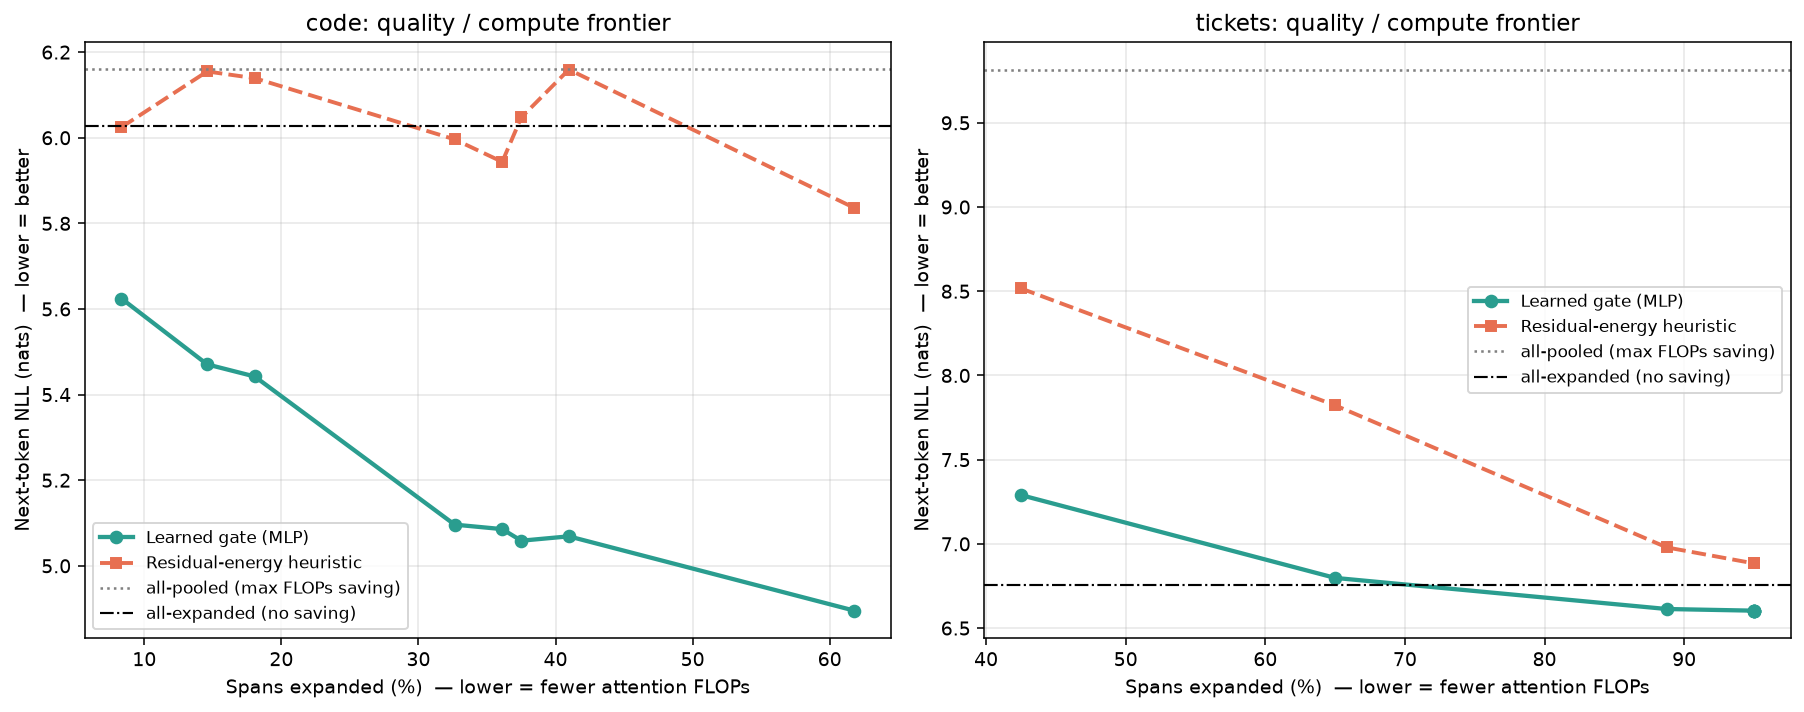
\includegraphics[width=0.92\textwidth]{gate_frontier.png}
\caption{Quality/compute frontier: learned gate (teal) vs.\ residual-energy heuristic
(orange), for code (left) and tickets (right). Lower NLL and fewer expanded spans are both
better. The learned curve lies entirely below the heuristic on both datasets; on code it
dips below the all-expanded reference (dash-dot), showing selective pooling can help.}
\label{fig:gate}
\end{figure}

\paragraph{Data-adaptivity.} The same mechanism behaves correctly across redundancy
regimes: where pooling is cheap (code) the gate is aggressively sparse; where pooling is
costly (tickets) it expands almost everything unless the sparsity pressure $\lambda$ is
large. The regularizer in Eq.~\eqref{eq:loss} thus acts as a direct, interpretable knob on
the compute/quality operating point.

\section{Wall-Clock Validation}
\label{sec:walltime}

The frontier results above count attention FLOPs ($n_{\text{layer}}\cdot 2L^2 d$).
A FLOPs count predicts a saving; it does not prove one on real hardware, where attention
is not the only cost: the MLP blocks, the language-model head, and the embedding lookups
are \emph{linear} in sequence length and do not shrink quadratically when spans are
collapsed. We therefore report \emph{measured} single-forward wall-clock time and peak
memory on CPU (2 vCPU, frozen models, no gradient), using warm-up passes and the median of
several repeats. All numbers in this section are realized, not estimated. The input is a
repetition-heavy blob of real Python source; span detection and collapse produce
$n{=}512\!\to\!m{=}340$.

\begin{table}[h]
\centering
\small
\begin{tabular}{lrrrr}
\toprule
Model & Params & Baseline (ms) & CTA (ms) & \textbf{Speedup} \\
\midrule
GPT-2 small  & 124M & 651  & 429  & \textbf{1.52$\times$} \\
GPT-2 medium & 355M & 1622 & 1070 & \textbf{1.52$\times$} \\
GPT-2 large  & 774M & 3529 & 2480 & \textbf{1.42$\times$} \\
\bottomrule
\end{tabular}
\caption{Measured wall-clock at fixed length (512 tokens). Span detection and \compose{}
add negligible overhead ($<0.3\%$ of CTA time). Peak RSS was 1.2/2.2/3.9\,GB respectively.
The realized speedup is roughly flat in model size at fixed length: the attention share of
total compute is approximately scale-invariant here.}
\label{tab:walltime-models}
\end{table}

The realized speedup does \emph{not} grow with model size at a fixed length, but it does
grow with \emph{length}, exactly as the quadratic attention term predicts. On GPT-2 small
the realized speedup rises monotonically from $1.29\times$ at 256 tokens to $1.71\times$ at
1024 (Table~\ref{tab:walltime-len}, Fig.~\ref{fig:walltime}) as attention comes to
dominate total compute. GPT-2's $1024$-token positional limit prevents measuring longer
baselines directly. (A quadratic-only FLOPs count would predict a larger ${\sim}2.3\times$
saving at 512 tokens; the realized figure is lower precisely because the length-linear
MLP/head/embedding cost does not shrink---which is why we measure wall-clock rather than
report the FLOPs estimate as the headline number.)

\begin{table}[h]
\centering
\small
\begin{tabular}{rrrrr}
\toprule
Length & $m$ & Baseline (ms) & CTA (ms) & \textbf{Speedup} \\
\midrule
256  & 193 & 319  & 246 & \textbf{1.29$\times$} \\
512  & 340 & 620  & 438 & \textbf{1.42$\times$} \\
768  & 485 & 1025 & 620 & \textbf{1.65$\times$} \\
1024 & 709 & 1339 & 784 & \textbf{1.71$\times$} \\
\bottomrule
\end{tabular}
\caption{Measured wall-clock speedup grows with sequence length (GPT-2 small): the
quadratic attention term becomes a larger share of total compute, so collapsing spans pays
off more.}
\label{tab:walltime-len}
\end{table}

\begin{figure}[t]
\centering
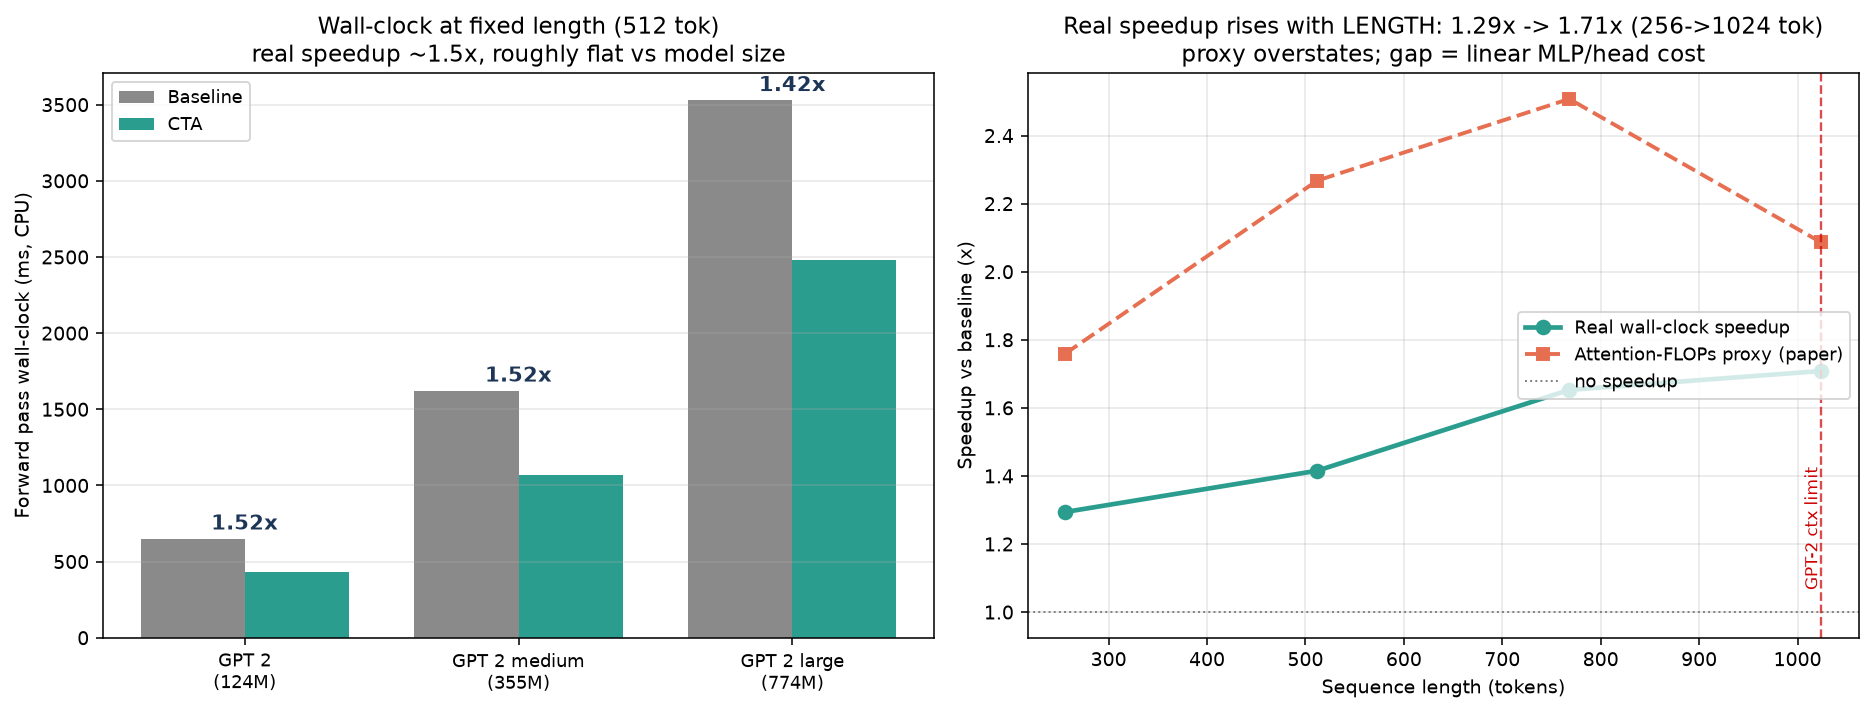
\includegraphics[width=0.92\textwidth]{walltime_results.png}
\caption{\textbf{Left:} measured wall-clock (baseline vs.\ CTA) at 512 tokens across the
GPT-2 size ladder; the speedup is ${\sim}1.5\times$ and roughly flat in model size.
\textbf{Right:} measured speedup vs.\ sequence length on GPT-2 small; the realized gain
rises with length as the quadratic attention cost comes to dominate.}
\label{fig:walltime}
\end{figure}

\subsection{Validation on a modern backbone (Qwen2.5)}
\label{sec:qwen}
Our main experiments use GPT-2, a reproducible but 2019-era backbone (learned positions, dense attention, 1024 context). To test that the mechanism is not tied to that architecture, we repeat the wall-clock measurement on Qwen2.5-0.5B (494M): a 2024 design with RoPE, grouped-query attention (14 heads / 2 KV heads), SwiGLU MLP and a 32k window. Because CTA operates purely on input embeddings, the port required no change to the algorithm---only a forward wrapper. Reversibility holds exactly ($3.73\times10^{-9}$, cleaner than GPT-2's $4.77\times10^{-7}$), and measured speedup again rises with length ($1.06\times$ at 256 to $1.58\times$ at 2048 tokens). The realized speedup is lower than GPT-2 at fixed length because Qwen has a deeper stack (24 vs 12 layers) and a much larger LM head ($\sim$152k vs $\sim$50k vocab), so the length-linear cost is a larger share of total compute.

\begin{table}[h]
\centering
\small
\begin{tabular}{rrrrr}
\toprule
Length & $m$ & Baseline (ms) & CTA (ms) & \textbf{Speedup} \\
\midrule
256  & 228  & 1079 & 1016 & \textbf{1.06$\times$} \\
512  & 421  & 2163 & 1942 & \textbf{1.11$\times$} \\
1024 & 727  & 4340 & 3176 & \textbf{1.37$\times$} \\
2048 & 1286 & 9010 & 5688 & \textbf{1.58$\times$} \\
\bottomrule
\end{tabular}
\caption{Measured wall-clock on Qwen2.5-0.5B (494M, 24 layers, $d{=}896$, RoPE + GQA + SwiGLU, 32k window), CPU, median of repeats. The mechanism ports unchanged; reversibility is exact ($3.73\times10^{-9}$) and the speedup rises with length, mirroring the GPT-2 trend. Qwen's 32k window lets us measure past the 1024-token GPT-2 ceiling.}
\label{tab:walltime-qwen}
\end{table}

\begin{figure}[t]
\centering
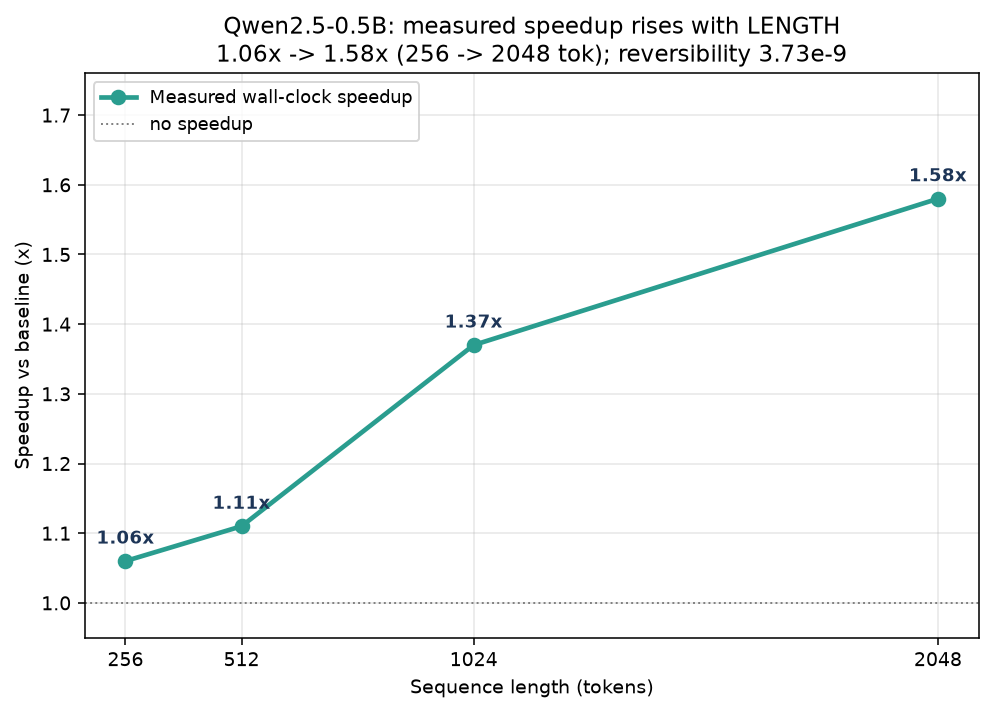
\includegraphics[width=0.62\textwidth]{qwen_walltime.png}
\caption{Measured wall-clock speedup vs.\ sequence length on Qwen2.5-0.5B. The same length-driven trend as GPT-2, extended to 2048 tokens; the realized gain is lower at fixed length because Qwen's deeper stack and larger head make the length-linear cost a bigger share of total compute.}
\label{fig:qwen}
\end{figure}

\paragraph{Bonus: effective context extension.} Because \compose{} shortens the sequence
losslessly, a context that overflows the model's positional window in full form can fit
after collapse. On the same corpus, up to ${\sim}1900$ raw tokens collapse to $m{\le}1024$
and thus \emph{fit} GPT-2's 1024-token window, where the baseline overflows outright---an
effective context extension of ${\sim}1.9\times$. This is a genuine, if corpus-dependent,
side benefit: the extension factor equals the achieved collapse ratio and therefore, like
the speedup, scales with the interchangeability of the context's repeats. It is not a
replacement for architectural long-context methods, and it degrades on shallow-redundancy
inputs where little collapse is possible.

\section{Discussion, Limitations, and Conclusion}
\label{sec:conclusion}

CTA reframes repeated spans as amortizable units of computation. Its defining property is
\emph{reversibility}: because $\compose$ is losslessly invertible, the model can operate on
a compact opaque sequence by default and pay for full resolution only where a learned,
compute-aware gate deems it necessary. Empirically, this yields a favorable frontier on
deep-redundancy data (code: $\sim\!50\%$ attention FLOPs at improved perplexity) and a
learned gate that strictly dominates a strong heuristic (up to $1.23$ nats).

\paragraph{Applicability boundary.} The central, honest finding is that CTA's benefit is
\emph{content-dependent}. On \emph{deep} redundancy---code, boilerplate, duplicated
prompts where repeated spans are truly interchangeable---collapse is nearly free and the
gate expands little. On \emph{shallow} redundancy---structured logs and tickets where a
repeated template (\texttt{"user\_id":}) immediately precedes distinguishing content
(the value)---pooling destroys exactly the predictive signal, and the gate must expand
aggressively, eroding the savings. CTA is therefore best understood not as a universal
compressor but as a mechanism whose gain scales with the \emph{interchangeability} of a
context's repeats.

\paragraph{Limitations.} (i) The gate is trained on \emph{marginal} per-span utility rather
than end-to-end through the full sequence, which is cheaper but less exact. (ii) Wall-clock
is measured on CPU only (Sec.~\ref{sec:walltime}): the realized speedup is ${\sim}1.5\times$
and grows with length; throughput on accelerators, with variable-length batching and
KV-cache reuse, remains to be measured. (iii)
The main qualitative experiments (reversibility, gated frontier, learned gate) use a small
frozen GPT-2 and modest, partly synthetic corpora. Wall-clock is additionally validated on
Qwen2.5-0.5B (RoPE + GQA + SwiGLU), where the mechanism ports without change and both
reversibility and the length-driven speedup trend are confirmed; validating the qualitative
results on larger modern models and held-out real corpora is future work. (iv) The gate's
query feature is a consumer-token embedding; the specification's $\gamma(q,\ebar)$ with $q$
a hidden state is strictly more expressive and requires intermediate activations.

\paragraph{Future work.} End-to-end gate training; per-layer CTA (expand in lower layers,
stay collapsed in upper layers, a dual-clock attention); composition with byte/patch
tokenizers (BLT, H-Net) treating patches as CTA atoms; and near-duplicate (semantic, not
just lexical) span classes via content-addressable attention.

\paragraph{Conclusion.} To our knowledge CTA is the first reversible, session-scoped,
parameter-free deduplication mechanism motivated by compute amortization. Reversibility
turns the classic lossy-merge dilemma into a per-query granularity choice, and a small
compute-aware gate learns to exploit it. The approach is a clear win where repeats are
interchangeable, and its limits are precisely characterized where they are not.

\begin{thebibliography}{9}
\small
\bibitem{blt} A.~Pagnoni et al. \emph{Byte Latent Transformer: Patches Scale Better Than Tokens.} arXiv:2412.09871, 2024.
\bibitem{hnet} S.~Hwang, B.~Wang, A.~Gu. \emph{Dynamic Chunking for End-to-End Hierarchical Sequence Modeling (H-Net).} arXiv:2507.07955, 2025.
\bibitem{asg} \emph{Breaking Token Into Concepts: Aggregate Semantic Grouping for Vocabulary Compression.} Findings of EMNLP, 2025.
\bibitem{r3mem} \emph{R3Mem: Bridging Memory Retention and Retrieval via Reversible Compression.} arXiv:2502.15957, 2025.
\bibitem{dtp} P.~Nawrot et al. \emph{Efficient Transformers with Dynamic Token Pooling.} ACL, 2023. arXiv:2211.09761.
\bibitem{tome} D.~Bolya et al. \emph{Token Merging: Your ViT But Faster.} ICLR, 2023. arXiv:2210.09461.
\bibitem{mtp} F.~Gloeckle et al. \emph{Better \& Faster Large Language Models via Multi-token Prediction.} ICML, 2024.
\end{thebibliography}

\end{document}
